\thispagestyle{fancy}
\begin{center}
	\LARGE{\textbf{Divisores de tensión}}
\end{center}
\section{Objetivos}
Al finalizar esta experiencia, usted estará capacitado para:
\begin{enumerate}
	\item	Calcular la salida de un divisor de tensión.
	\item Comprobar el principio del divisor de tensión por medición directa.
	
\end{enumerate}
\section{Conocimientos previos}
El divisor de tensión es una red de resistores utilizada para reducir una tensión a un valor menor de acuerdo a las necesidades específicas. La ecuación para calcular la caída de tensión a través de la resistencia de la salida es:
\begin{equation*}
	V_{sal}= \frac{R_{sal}}{R_{total}}*V_{entrada}
\end{equation*}
\section{Autoevaluación de entrada}
\begin{enumerate}
	\item	La tensión en la salida en un divisor de tensión es: Menor que la fuente de tensión.
	\item Cuando se incrementa la resistencia de la salida, la tensión de salida: Se incrementa
	
\end{enumerate}
\section{Equipo}
El siguiente equipo es necesario para la realización del experimento.
\begin{enumerate}
	\item 	Módulo de experimentación
	\item 	DMM (Multímetro digital)
\end{enumerate}
\section{Procedimiento}
Para comprobar sus habilidades en la resolución de problemas, puede utilizar
simuladores como multisim, Ud. Puede, si lo desea, añadir componentes e
instrumentos de medición, y comprobar los resultados.
\begin{enumerate}
	\item 1.	Efectué los cálculos necesarios para el circuito de la figura 9.1
	\begin{figure}[h]
		\centering
		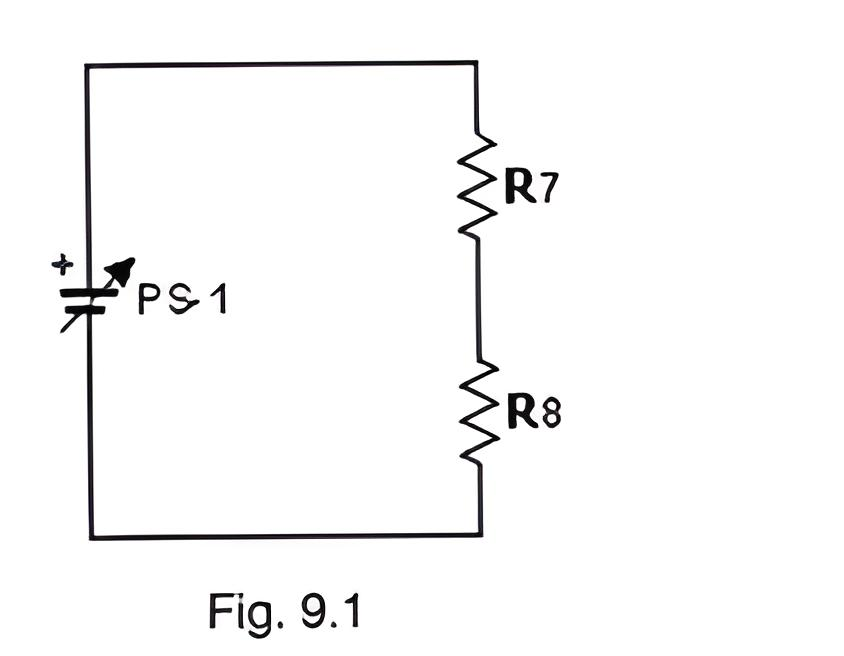
\includegraphics[scale=0.2]{imagenes/1}
	\end{figure}
	\item	Implemente el circuito que contiene los resistores R7 y R8, como se muestra en la figura 9.1
	\item 	Lleve las tensiones de ambas fuentes a 0V. Conecte R7 y R8 como divisores de tensión.
	\item Lleve la salida de PS-1 a 7.5 V. Use el DMM para medir la tensión de la fuente y en bornes de R8. Anote ambos valores en la tabla 9.1
	\item Utilizando la ecuación de divisores de tensión, calcular la tensión teórica de salida usando R8 como resistencia de salida, y R7+R8 como la resistencia total. Registre los resultados en la tabla 9.1
	\begin{figure}[h]
		\centering 
		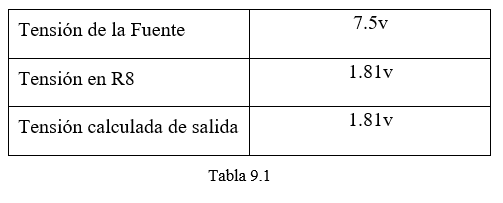
\includegraphics[scale=1.2]{imagenes/2}
	\end{figure}
	\item 	Lleve la salida de PS1 a 0V y desconecte el circuito. Estudie el circuito e la figura 9.2
	\item	Conecte el circuito como se muestra en la figura 9.2
	\item	Lleve la salida PS-1 a 8V. Mida y registre la tensión de salida del divisor(sobre R8
	\begin{figure}[h]
		\centering
		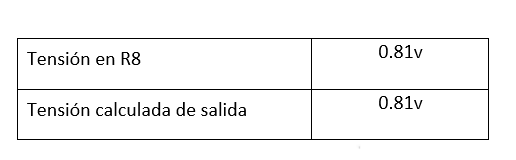
\includegraphics[scale=1.2]{imagenes/3}
	\end{figure}
	\item 	Calcule la salida del divisor usando la ecuación del divisor de tensión.
	\begin{equation*}
		V_{sal}= \frac{R_{sal}}{R_{total}}*V_{entrada}
	\end{equation*}
	\begin{equation*}
		V_{sal}= \frac{1500}{14800}*V_{8}
	\end{equation*}
	\begin{equation*}
		V_{sal}=0.8108V
	\end{equation*}
\end{enumerate}
\section{Autoevaluación}
\begin{enumerate}
	\item 	Dada una fuente de tensión 12V y seis resistores de 1KΩ en serie, se desea obtener una referencia de tensión de 4V. La salida es tomada sobre:
	6KΩ
	\item	Dos resistencias de 5.1KΩ y 2,2KΩ conectados en serie a través de una batería de 12V. La tensión en el resistor de 2,2KΩ será:
		\begin{equation*}
		V_{sal}= \frac{R_{sal}}{R_{total}}*V_{entrada}
	\end{equation*}
	\begin{equation*}
		V_{sal}= \frac{2.2}{7.3}*V_{8}
	\end{equation*}
	\begin{equation*}
		V_{sal}=3.62V
	\end{equation*}
	
\end{enumerate}
\section{Conclusiones}
Se demuestra la importancia de comprender como se distribuye la tensión en un circuito y cómo las resistencias afectan el comportamiento global del circuito.


